\documentclass[12pt,journal,compsoc, a4paper, onecolumn]{IEEEtran}
\usepackage{applekeys}
\usepackage[utf8]{inputenc}
\usepackage{hyperref} 
\usepackage{fancyhdr}
%\usepackage{graphicx}



\begin{document}

\title{CodeLab \\ Design Document}

\author{Bjørn~Fjukstad \\ BIO-8010 Communicating Science Module 3\\ Visualizing
your science \\ \url{github.com/fjukstad/bio-8010}} 

\maketitle
\vspace{-15mm}

\section{Introduction} 
CodeLab is a game where kids collaborate on escaping from an underground
dungeon by programming their in-game characters to fight monsters, solve puzzles
and collect gems. The game is played in a collaborative environment such as the
Tromsø Display Wall\cite{anshus2013nineyears}, where kids program on their own
devices and run the game on a large shared display. The display wall environment
provides an interactive arena where kids can collaborate on completing the game
together.

Since the kids need to program the characters to perform different tasks, they
will have to learn the basics of programming. The different levels will require
them to learn about \emph{variables}, \emph{data structures}, \emph{functions}
and \emph{control statements} such as \emph{for}-loops and \emph{if}-statements. 
As the kids play the game, the puzzles and problems they are faced with will
increase in difficulty, making it necessary to design and implement more
complex solutions. 

The game is intended for children 10 - 16 years old, who already have some
experience with graphical programming environments such as
Scratch\cite{resnick2009scratch}. It is intended for kids that want to learn
more about programming, specifically getting started with text-based
programming. 

CodeLab is open-sourced at \url{github.com/fjukstad/bio-8010} and there is a
playable prototype of the first-level at \url{fjukstad.github.io/bio-8010}. 

% Structure
%\subsection{Concept, Goal and Learning Goals} 
%\subsection{Target Audience} 

\section{Background} 
For teaching programming to children there exists a plethora of different
systems and tools. For the youngest kids, a popular alternative is
Scratch\footnote{\url{scratch.mit.edu}}, where kids use a visual programming
language where they can make games and other small projects.  For older kids a
popular choice is to go into game modding, specifically modding the popular
video game MineCraft\footnote{\url{minecraft.net}}.
CodeCombat\footnote{\url{codecombat.com}} is another alternative where kids
program game characters through labyrints or different set of tasks. If kids
want a more hands-on approach it is popular to program either Lego
Mindstorms\footnote{\url{mindstorms.lego.com}} or small Arduino
computers\footnote{\url{arduino.cc}}. 

CodeLab is a game that tries to make learning text-based programming more fun
and collaborative through a video game that kids play in an shared environment.
It takes the gameplay from its competator CodeCombat and the physical hands-on
interaction from Lego Mindstorms and Arduinos, making an interactive and
collaborative learning environment for programming. 

\section{Description} 
CodeLab takes place in a fictional dungeon, where each player is assigned a
hero that he or she controls by programming their actions. The players equip
their heroes with armor, weapons and other items that can help them complete the
different levels. For each level, the players have to complete a set of tasks by
programming their characters by using a programming language similar to the 
Lua programming language\footnote{\url{lua.org}}. Players 
write the code on their local machine, be it a laptop or a smart phone, and see
their characters perform the actions on a large shared display. Alongside the
game view, the players see each others code making it possible to help out
eachother if they encounter any problems. 

The game is turn-based in the sense that every turn is a line of code or the
execution of a program. The players can either run their entire program to pass
the level, or they can interactively type commands that completes the level.
Typically the first levels where the players would only move a character is
suitable for an interactive solution, while later levels require more complex
programs that are difficutly to complete by writing only single lines at a time. 

\subsection{Game Narrative} 
The game starts with the players being introduced to their heroes and the
dungeon they find themselves in. The players get to know what they can equip
their heroes with and the actions they can make their heroes do. Each set of
item has special actions that the players can use, e.g. you need to equip a hero
with boots if you want him to move. Some boots give you the power to walk
faster, while some give you the ability to climb obstacles. The players are also
introduced to the programming that they need to do to complete every level. The
first level introduces them to the four commands: $moveDown$, $moveUp$,
$moveRight$ and $moveLeft$ that moves their character either down, up, right or
left. Figure 1 shows a sketch of the first level. The player is the blue circle,
and the goal of the level is to navigate down to the yellow square.  In the full
game you would image that the circle is replaced with a more graphical game
character, and that the yellow square could be a person that needs help or
assistance. 

\begin{figure}[htb!]
    \begin{centering}
    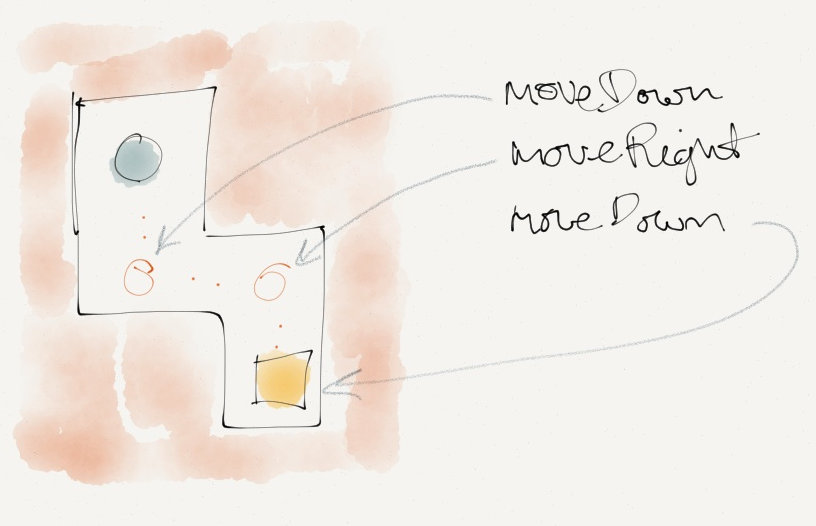
\includegraphics[width=0.6\textwidth]{./figures/codelab3.png}
    \caption{A sketch of the first level of CodeLab. The goal of the level
    is to write code that moves the character (the circle) down to the
    yellow square. The player writes three commands, $moveDown$,
    $moveRight$ and $moveDown$ to complete the level. } 
    \label{fig:level1}
    \end{centering} 
\end{figure}


In the first stages of the game the players would also need to familiarize
themselves in the game setting. CodeLab is designed to run in a collaborative
environment such as the Tromsø Display Wall, where each player writes code on
their own device while the graphical output of game is shown on a large shared
display. This encourages collaboration between the players, and creates a more
interactive learning environment for the children playing the game. From my
experience with the local Code Club, having something run in a shared setting
makes the whole coding experience more fun and collaborative than working on
your own computer. 

As the game progresses both the difficulty of the levels and the complexity of
the code the players produce increase. The first levels will concentrate on the
basics of programming, with different commands that the players can execute.
Following these the players are introduced to \emph{conditionals} such as
\emph{if}-statements or \emph{for}-loops, \emph{data structures} and
\emph{variables}, and \emph{functions}. As the game progresses the players will
have access to more commands and features, such as the ability to fight
monsters, build structures and forge weapons. 

The ultimate goal of the game is to escape the dungeon that the player is
trapped in, and have learned the basic skills needed to get started with
text-based programming. 

\subsection{Game Environment} 
Figure \ref{fig:environ} shows an illustration of the shared environment CodeLab
I envision children playing the game in. Kids collaborate on writing the code
that makes it possible to complete a level. They can write the code on their own
devices, but must run the game on the shared display where other kids can view
their progress and code. 

\begin{figure}[htb!]
    \begin{centering}
    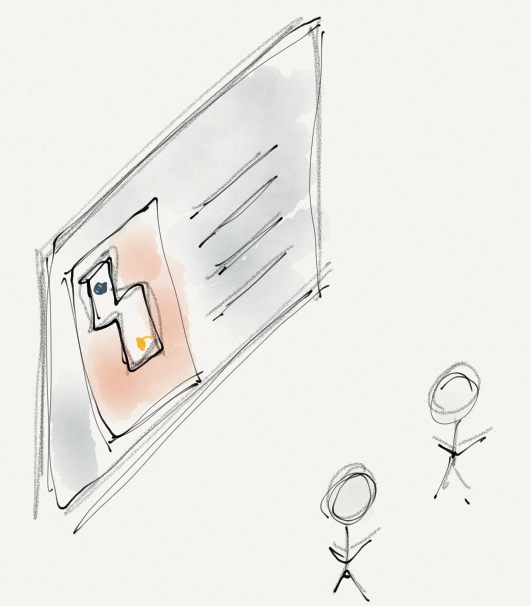
\includegraphics[width=0.5\textwidth]{./figures/codelab2.png}
    \caption{The CodeLab environment. Players collaborate to solve a level. Both
    the graphical window where the game runs, as well as the source code is
    shown on a large display. } 
    \label{fig:environ}
    \end{centering} 
\end{figure}

In addition to just having one game session on the shared display, some levels
of CodeLab requires that kids collaborate to continue to the next level. Figure
\ref{fig:2p} illustrates how players are given similar levels that they have to
complete together to proceed.  Collaborating on the different levels will help
the kids learn more about the collaborative side of programming by sharing code
and helping others. 

\begin{figure}[htb]
    \begin{centering}
    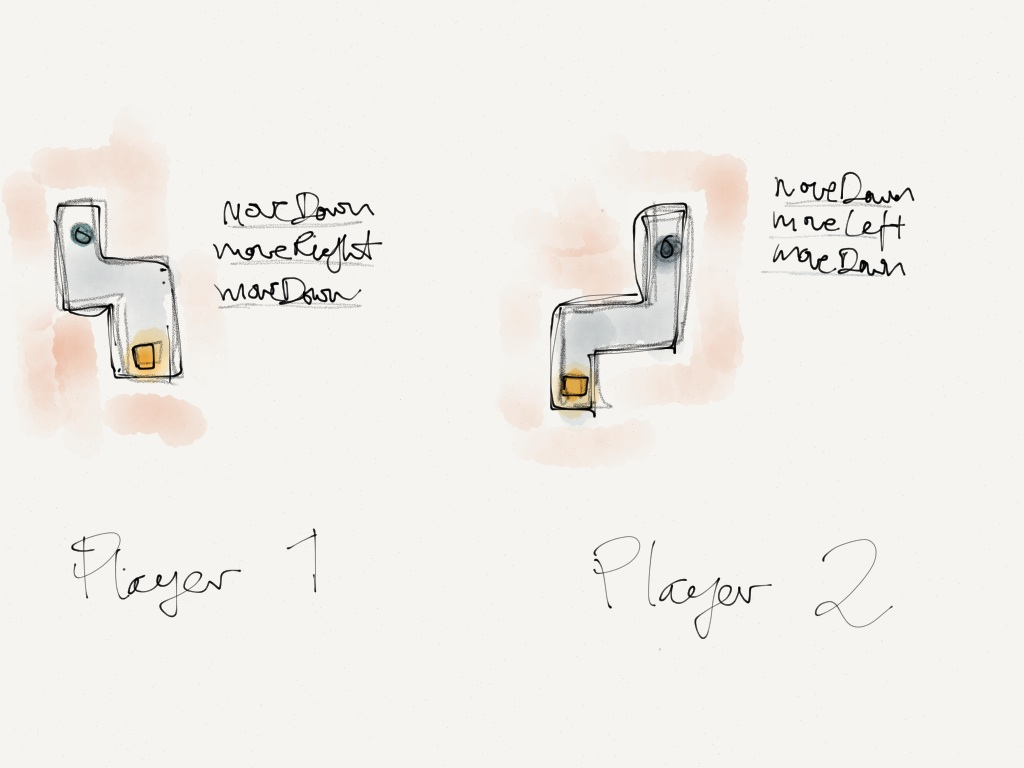
\includegraphics[width=0.6\textwidth]{./figures/codelab5.jpg}
    \caption{Two players trying to complete the first level. This view is shown
    on the large display, where they can help each other write the necessary
    code. } 
    \label{fig:2p}
    \end{centering} 
\end{figure}

\subsection{Game Tasks} 
The overall goal of CodeLab is to escape the dungeon that our heres has fallen
into, and by doing so learning text-based programming. The game itself is broken
into smaller levels that the players need to complete by programming the actions
of their characters. Every level will have one or more specific goals that the
game characters have to complete, e.g. defeat an enemy or get to a specific
location. Some levels will also require that the players use specific
programming skills, such as placing actions within a \emph{for}-loop or a
\emph{function}. 


\section{Game Mechanics} 
CodeLab is in essence two games in one. The first being the actual dungeon where
the heroes live, where they must fight enemies and ultimately escape. The other
is the coding-part where kids use their skills to control their heroes through
real programming. These are tightly coupled to each other, new items allow the
players to use new functions and so on. 

The game within code lab is a role playing game where the characters wear armor
and fight enemies with swords, spears and other medieval weapons. They move in a
two-dimensional world from the input commands that the players run, making it
possible to move up/down/left/right and jump. The levels are tile-based making
it possible to move one tile per command. If the players gain any power-ups it
will be possible to move faster, and also jump over tiles. Moving faster and
jumping will require special power-ups or special equipment. 

If the characters encounter enemies they will have to use their weapons to kill
them. If the heroes unfortunately die, they will have to start the level over
again, but they won't loose any equipment or loose the code that they have
written for the level. On every level the heroes start off with some amount of
health points (HP). Protective clothing or armor will increase this number, and
this will be needed to pass some levels. 

Some levels will also require the players to build structures such as walls to
keep enemies away, or structures such as bridges to cross obstacles like rivers.
These structures are built by placing different blocks (like in Minecraft) onto
the level. 

\subsection{Progression} 
As the players play the game both the levels themselves and the programming to
complete them get more complex. The first levels can be completed using simple
functions, but later levels will require the payers to use control statements
such as \emph{if}-tests or \emph{for}-loops. In Figure \ref{fig:loop} we see a
level that will force the players to learn about loops. The level can be
completed by writing three series of $moveDown$, $moveRight$, $moveUp$ and
$moveRight$ commands, but the level will not accept any code that doesn't have
these within a loop. 

\begin{figure}[htb]
    \begin{centering}
    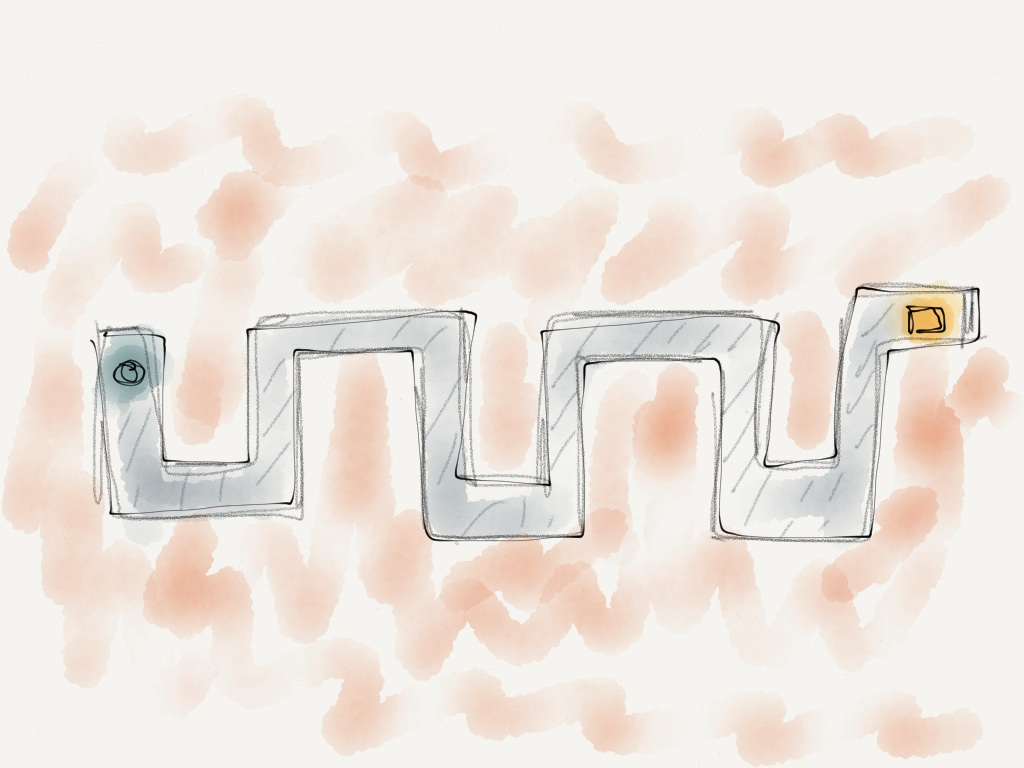
\includegraphics[width=0.6\textwidth]{./figures/codelab4.jpg}
    \caption{A level that can be completed by writing a simple loop.} 
    \label{fig:loop}
    \end{centering} 
\end{figure}

As the players complete levels they will unlock new ones and improve their own
hero by leveling them up and unlocking new features. Some levels is only
possible to unlock if the players have written enough code, and some will
require the players to equip special items to their characters.

When the players reach the end of the game they will have an entire arsenal of
programming constructs and commands to choose from. The later levels will
require the players to be more creative in how they solve problems, and will
give little or no instructions on how to solve problems to complete levels. 


\subsection{Reward and Motivation} 
As the game progresses the players will receive items that they can equip their
heroes. They will also receive rewards for writing clean code in form of gold
that they can use to purchase items. Players will be rewarded more for cleaner
code, and will motivate them to improve their code-writing skills. 

\subsection{Balancing} 
It is important that the levels provide sufficient challenges for the players so
that they want to continue to the next level. It will be necessary to learn
different programming constructs in different settings, so making levels that
test the same skills must be different from each other. Just moving a character
can get repetative, so each level should introduce something new in terms of
challenges to the player. Designing how the levels change will require balacing
and testing the game with actual players. 

\section{Platform} 
In CodeLab the choice of platform is very important. CodeLab runs in a shared
environment where the players can collaborate and cooperate on completing
levels. It should run on the Tromsø Display Wall or a similar setup, where there
is a large high resolution display for displaying a lot of content. In
the Display Wall lab you would connect your own device, such as an iPad or
laptop, to the local network and the large display where the game is run.
The game itself runs in a web browser, so that players don't need to install
anything to get it up and running. This is an important part since kids are
going to play the game, and do not necessarily have the access rights to install
applications or games. 

\subsection{Art} 
CodeLab uses a cartoonish art theme, with inspiration from games such as Skyrim
and MineCraft. Since it takes place in a dungeon the colors will be grey-ish,
but keeping the colors bright and welcoming. It will use bright blue colors for
water and warm red colors for lava to spice up the game. 

\subsection{Music and Audio}
Music and other audible elements is important to make a more complete gaming
experience. Since players must concentrate on writing code to complete each
level, the background music should be toned down to almost a minimum. However as
the players complete their code and want to run it, it should increase the
intensity of the music to make the experience more exiting. CodeLab should also
include in-game audio from the characters and their surrondings. 

\section{Production and Team} 
To make CodeLab a reality we would need a team of at least to persons, one
artist and one programmer. Making a really simple prototype only took about a
day, including the time to get it running on the Troms{\o} Display Wall, but to
make something that can be used to sell the game to potential investors would
include a couple of weeks. To test the game it could have been introduced in the
local Code Club, so that developers could get feedback on what works and what
doesn't.  

\section{Prototype} 

To try out how the actual game would work in practice, I wrote a small
prototype. The prototype is available to try out at
\url{fjukstad.github.io/bio-8010} and runs in a web browser. The game is written
in Javascript and uses the Javascript library D3\footnote{\url{d3js.org}} to
draw the basic graphics. To input the commands ($moveUp()$, $moveDown()$,
$moveLeft()$, $moveRight()$) to move the circles, players
need to open the Developer Console (\cmdkey+\optkey+j in Chrome on a Mac).
Figure \ref{fig:real1} shows the first level running on the display wall.
Unfortunately the prototype does not show the active commands from the user, but
we plan to place them adjacent to the game area on the left. Figure
\ref{fig:real2} shows the output when the player has completed the level. 

\begin{figure}[htb]
    \begin{centering}
    \includegraphics[width=0.6\textwidth]{./figures/codelab-real1.jpg}
    \caption{The first level of the prototype running on the Tromsø Display
    Wall. The black squares are projectors that unfortunately did not work on
the day we tried the prototype. Off-screen is the player typing commands to move
the blue circle. } 
    \label{fig:real1}
    \end{centering} 
\end{figure}

\begin{figure}[htb]
    \begin{centering}
    \includegraphics[width=0.6\textwidth]{./figures/codelab-real2.jpg}
    \caption{The first level completed on the Tromsø Display Wall} 
    \label{fig:real2}
    \end{centering} 
\end{figure}

\section{Acknowledgements}
Thanks to Jason Tang for getting the CodeLab prototype to run on the Troms{\o}
Display Wall. 

% Fetch your references, in a file called report.bib
\bibliography{design-document}{}
\bibliographystyle{plain}
\end{document} 
